\documentclass[14pt]{extarticle}
\usepackage{fontspec}
\usepackage{polyglossia}
\usepackage{amsmath}
\usepackage{amssymb}
\usepackage{xcolor}
\usepackage{fancyhdr}
\usepackage{graphicx}
\usepackage{listings}
\usepackage[most]{tcolorbox}
% \usepackage{setspace}
\usepackage{pifont}
\usepackage{enumitem}
\usepackage{titlesec}
\usepackage[bottom]{footmisc}
\usepackage{titling}
\usepackage{minted}
\usepackage{etoolbox}
\usepackage{array}
\usepackage{extsizes}
\usepackage{float}
\usepackage{booktabs}
\usepackage{hyperref}
\usepackage[onehalfspacing]{setspace}
\usepackage[a4paper, top=2.7cm, bottom=2.7cm, left=2.5cm, right=2.5cm, headheight=1.5cm, headsep=0.5cm]{geometry}
\usepackage{tikz}

\usetikzlibrary{automata, positioning, arrows.meta, arrows}

\newfontfamily\emoji{Segoe UI Emoji}

\pagestyle{fancy}

\setmainlanguage[numerals=western]{arabic}
\setotherlanguage{english}
% \newfontfamily\arabicfont[Script=Arabic]{Amiri}
\newfontfamily\arabicfont[Script=Arabic]{Calibri}
\newfontfamily\arabicfonttt[Script=Arabic]{Courier New}

\lstset{
  language=[Sharp]C,
  numbers=left,
  stepnumber=1,
  numbersep=8pt,
  frame=single,
  basicstyle=\ttfamily\small,
  keywordstyle=\color{blue},
  stringstyle=\color{red},
  commentstyle=\color{green!50!black}
}

\newif\ifdetailed
\ifdefined\setdetailed
  \setdetailed
\fi

\newif\ifwithsols
\ifdefined\setwithsols
  \setwithsols
\fi

% unified tcolorboxes for articles
\tcbset{colback=white, colframe=black, fonttitle=\bfseries, boxrule=0.8pt}
\newtcolorbox{boxDef}[1][]{colback=blue!5!white,colframe=blue!75!black,
  title={{\emoji📘} تعريف\ifx\\#1\\\else ~#1\fi :}}
\newtcolorbox{boxExercise}[1][]{colback=cyan!5!white,colframe=cyan!70!black,
  title={{\emoji🧩} تمرين\ifx\\#1\\\else ~#1\fi :}}
\newtcolorbox{boxExample}[1][]{colback=yellow!5!white,colframe=orange!90!black,
  title={{\emoji📝} مثال\ifx\\#1\\\else ~#1\fi :}}
\newtcolorbox{boxNote}[1][]{colback=gray!10!white,colframe=black,
  title={{\emoji✨} ملاحظة\ifx\\#1\\\else ~#1\fi :}}
\newtcolorbox{boxAttention}[1][]{colback=magenta!10!white,colframe=magenta!80!black,
  title={{\emoji🔔} تنبيه\ifx\\#1\\\else ~#1\fi :}}
\newtcolorbox{boxWarning}[1][]{colback=red!5!white,colframe=red!75!black,
  title={{\emoji⚡} ملاحظة هامة\ifx\\#1\\\else ~#1\fi :}}
\newtcolorbox{boxSolution}[1][]{colback=green!5!white,colframe=green!60!black,
  title={{\emoji✅} حل\ifx\\#1\\\else ~#1\fi :}}
\newtcolorbox{boxSymbol}[1][]{colback=purple!5!white,colframe=purple!70!black,
  title={{\emoji🔣} رمز\ifx\\#1\\\else ~#1\fi :}}
\newtcolorbox{boxHint}[1][]{colback=teal!5!white,colframe=teal!60!black,
  title={{\emoji💡} تلميح\ifx\\#1\\\else ~#1\fi :}}


\tcbset{simplecode/.style={ colback=gray!5, colframe=black!50, boxrule=0.4pt, arc=2pt, left=4pt,right=4pt,top=4pt,bottom=4pt}}
\newenvironment{boxCode}{\begin{tcolorbox}[simplecode]}{\end{tcolorbox}}

\newcolumntype{C}[1]{>{\centering\arraybackslash}p{#1}}

% redefine spaces after titles
\makeatletter
\renewcommand{\@maketitle}{%
  \begin{center}
    {\huge \bfseries \@title \par}%
    \vskip 0.2em % space between title and author
    {\large \@author \par}%
    % \vskip 0.2em % space between author and date
    % {\normalsize \@date \par}%
  \end{center}
}
\makeatother

\fancyhf{} % clear default
\fancypagestyle{plain}{
  \fancyhf{}
  \fancyhead[L]{مدرسة التسامح الشاملة}
  % \fancyhead[L]{
\includegraphics[height=1cm]{../../../images/logoTasamoh.png}}
  \fancyhead[R]{الأستاذ محمود اغبارية}
  \fancyfoot[C]{\thepage}
}

\fancyhead[L]{مدرسة التسامح الشاملة}
\fancyhead[R]{الأستاذ محمود اغبارية}
\fancyfoot[C]{\thepage}
% \date{\today}

\setcounter{tocdepth}{3} % only section subsection and subsubsection in TOC

\newcommand{\importpdfpage}[2]{%
    \thispagestyle{empty}
    \newgeometry{left=0cm,right=0cm,top=0cm,bottom=0cm}
    \includegraphics[page=#2,width=0.95\paperwidth,height=0.95\paperheight,keepaspectratio]{#1}
    \restoregeometry
}

\newcommand{\insertFullImg}[1]{%
    \noindent
    \makebox[\textwidth][c]{
        \includegraphics[width=0.9\paperwidth,keepaspectratio]{#1}%
    }%
}%

% ----------------------


% \begin{document}

% \maketitle

% % \clearpage  % start TOC on a new page
% % \renewcommand{\contentsname}{جدول المحتويات}
% % \tableofcontents
% % \clearpage

% \part*{part 1} % the * prevents numbering
% \section*{مقدمة}
% \subsection*{مثال رياضي}
% \subsubsection*{مثال فرعي}
% \paragraph*{ paragraph 1}
% \subparagraph*{sub paragraph 1}

% \ifdetailed
% \begin{english}
% \begin{minted}{csharp}
% // C# Example
% \end{minted}
% \end{english}
% \fi

% OLD WAY
% \ifdetailed
% \begin{english}
% \begin{lstlisting}
% // C# Example
% \end{lstlisting}
% \end{english}
% \fi

% % 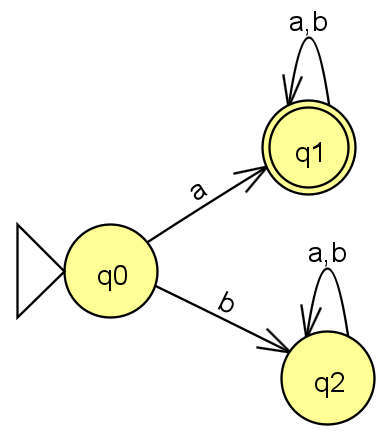
\includegraphics[width=0.2\textwidth]{../../../images/DFAs/ex1_q1.png}



% \vspace{3cm}
% \begin{flushleft}
% أرجو لكم وقتًا ممتعًا.

% الأستاذ محمود اغبارية.
% \end{flushleft}


% \end{document}


\ifwithsols
\title{حل وظيفة 14 - المصفوفات الأحادية - أسئلة متقدمة}
\else
\title{وظيفة 14 - المصفوفات الأحادية - أسئلة متقدمة}
\fi

\begin{document}

\maketitle
\thispagestyle{fancy}

\begin{enumerate}[itemsep=2em]


    \item اكتب عملية خارجية \textenglish{CountGreaterThanPrevious} تتلقى مصفوفة أعداد صحيحة وتعيد عدد العناصر التي هي أكبر من العنصر السابق لها في المصفوفة. \\
    \textbf{مثال:} في المصفوفة \textenglish{\{3, 5, 2, 8, 6\}} تعيد العملية 2 لأنّ:
    \begin{itemize}[itemsep=1pt]
        \item 5 أكبر من 3 (تحتسب)
        \item 2 ليس أكبر من 5 (لا تحتسب)
        \item 8 أكبر من 2 (تحتسب)
        \item 6 ليس أكبر من 8 (لا تحتسب)
    \end{itemize}
    \ifwithsols
    \begin{boxSolution}
    \begin{english}
    \begin{minted}{csharp}
public static int CountGreaterThanPrevious(int[] arr)
{
    int count = 0;
    for (int i = 1; i < arr.Length; i++)
    {
        if (arr[i] > arr[i - 1])
            count++;
    }
    return count;
}
    \end{minted}
    \end{english}
    \end{boxSolution}
    \clearpage
    \fi

    \item
    اكتب عملية خارجية \textenglish{SumArraysReverse} تتلقى مصفوفتي أعداد صحيحة لهما نفس الحجم، وتعيد مصفوفة جديدة بنفس الحجم تحتوي على مجموع عناصر من المصفوفتين بالشكل التالي:
    \begin{itemize}
        \item العنصر الأول في المصفوفة الجديدة هو مجموع العنصر الأول من المصفوفة الأولى والعنصر الأخير من المصفوفة الثانية.
        \item العنصر الثاني في المصفوفة الجديدة هو مجموع العنصر الثاني من المصفوفة الأولى والعنصر قبل الأخير من المصفوفة الثانية.
        \item وهكذا...
    \end{itemize}
    \textbf{مثال:} إذا كانت المصفوفة الأولى \textenglish{\{1, 2, 3\}} والمصفوفة الثانية \textenglish{\{4, 5, 6\}}، فإن المصفوفة الجديدة ستكون \textenglish{\{1 + 6, 2 + 5, 3 + 4\}} أي \textenglish{\{7, 7, 7\}}.
    \ifwithsols
    \begin{boxSolution}
    \begin{english}
    \begin{minted}{csharp}
public static int[] SumArraysReverse(int[] arr1, int[] arr2)
{
    int[] result = new int[arr1.Length];
    for (int i = 0; i < arr1.Length; i++)
    {
        result[i] = arr1[i] + arr2[arr2.Length - 1 - i];
    }
    return result;
}
    \end{minted}
    \end{english}
    \end{boxSolution}
    \clearpage
    \fi

    \item اكتب عملية خارجية \textenglish{MoveNegativesToEnd} تتلقى مصفوفة أعداد صحيحة وتعيد مصفوفة جديدة تحتوي على نفس العناصر ولكن مع نقل جميع الأعداد السالبة إلى نهاية المصفوفة.
    \textbf{مثال:} في المصفوفة \textenglish{\{3, -1, 4, -2, 5\}}، النتيجة ستكون \textenglish{\{3, 4, 5, -1, -2\}} أو أي ترتيب آخر للعناصر الموجبة في البداية والعناصر السالبة في النهاية.

    \ifwithsols
    \begin{boxSolution}
    \begin{english}
    \begin{minted}{csharp}
public static int[] MoveNegativesToEnd(int[] arr)
{
    int[] result = new int[arr.Length];
    int index = 0;
    for (int i = 0; i < arr.Length; i++)
    {
        if (arr[i] >= 0)
        {
            result[index] = arr[i];
            index++;
        }
    }
    for (int i = 0; i < arr.Length; i++)
    {
        if (arr[i] < 0)
        {
            result[index] = arr[i];
            index++;
        }
    }
    return result;
}
    \end{minted}
    \end{english}
    \end{boxSolution}
    \clearpage
    \fi

    {\large\textbf{سؤال بونوس:}} قم بنفس المهمة لكن على نفس المصفوفة دون الاستعانة بمصفوفة جديدة، أي تكون العملية: \textenglish{void MoveNegativesToEnd(int[] arr)}.
    \ifwithsols
    \begin{boxSolution}[البونوس]
    \begin{english}
    \begin{minted}{csharp}
public static void MoveNegativesToEnd(int[] arr)
{
    int pos = 0, neg = arr.Length - 1;
    while(pos < neg)
    {
        if (arr[pos] >= 0)
            pos++;
        if (arr[neg] < 0)
            neg--;
        if(arr[pos] < 0 && arr[neg] >= 0)
        {
            int temp = arr[pos];
            arr[pos] = arr[neg];
            arr[neg] = temp;
            neg--;
            pos++;
        }
    }
}
    \end{minted}
    \end{english}
    \end{boxSolution}
    \fi
\end{enumerate}

\end{document}
